

%% AP Physics MC Questions Archive
%%----------------------------------------


%% Projectile Motion
%%----------------------------------------
\element{ap}{
\begin{question}{projectile-motion-q01}
    %Base your answers to questions 1 and 2 on the following information.
    An object is thrown off a cliff above level ground with an initial horizontal velocity of \SI{15}{\meter\per\second}.
    It takes \SI{4}{\second} for the object to reach the ground.
    %% Start question
    If air resistance is negligible,
        the height of the cliff is most nearly:
    \begin{multicols}{3}
    \begin{choices}
        \wrongchoice{\SI{60}{\meter}}
      \correctchoice{\SI{80}{\meter}}
        \wrongchoice{\SI{120}{\meter}}
        \wrongchoice{\SI{160}{\meter}}
        \wrongchoice{\SI{240}{\meter}}
    \end{choices}
    \end{multicols}
\end{question}
}

\element{ap}{
\begin{question}{projectile-motion-q02}
    %Base your answers to questions 1 and 2 on the following information.
    An object is thrown off a cliff above level ground with an initial horizontal velocity of \SI{15}{\meter\per\second}.
    It takes \SI{4}{\second} for the object to reach the ground.
    %% Start question
    If air resistance is negligible,
        the distance from the base of the cliff that the object lands is most nearly:
    \begin{multicols}{3}
    \begin{choices}
      \correctchoice{\SI{60}{\meter}}
        \wrongchoice{\SI{80}{\meter}}
        \wrongchoice{\SI{120}{\meter}}
        \wrongchoice{\SI{160}{\meter}}
        \wrongchoice{\SI{240}{\meter}}
    \end{choices}
    \end{multicols}
\end{question}
}

\element{ap}{
\begin{question}{projectile-motion-q03}
    An object is thrown off of a cliff above ground level with an initial upward velocity of \SI{6}{\meter\per\second},
        and an initial horizontal velocity of \SI{15}{\meter\per\second}.
    It takes \SI{3}{\second} for it to reach the ground.
    If air resistance is neglected,
        the height of the cliff is most nearly:
    \begin{multicols}{3}
    \begin{choices}
        \wrongchoice{\SI{18}{\meter}}
      \correctchoice{\SI{27}{\meter}}
        \wrongchoice{\SI{45}{\meter}}
        \wrongchoice{\SI{63}{\meter}}
        \wrongchoice{\SI{90}{\meter}}
    \end{choices}
    \end{multicols}
\end{question}
}

\element{ap}{
\begin{question}{projectile-motion-q04}
    An object is thrown horizontally off of a \SI{125}{\meter} high cliff above level ground with an initial velocity of \SI{15}{\meter\per\second}.
    If air resistance is negligible,
        the distance from the base of the cliff to the point where the object lands is most nearly:
    \begin{multicols}{3}
    \begin{choices}
        \wrongchoice{\SI{25}{\meter}}
        \wrongchoice{\SI{45}{\meter}}
      \correctchoice{\SI{75}{\meter}}
        \wrongchoice{\SI{90}{\meter}}
        \wrongchoice{\SI{150}{\meter}}
    \end{choices}
    \end{multicols}
\end{question}
}

\element{ap}{
\begin{question}{projectile-motion-q05}
    %Base your answers to questions 5 and 6 on the following information.
    An object is thrown with a horizontal velocity of \SI{15}{\meter\per\second} off of a cliff that is \SI{180}{\meter} above level ground.
    %% Start Question
    If air resistance is negligible,
        the time it takes the object to reach the ground is most nearly:
    \begin{multicols}{3}
    \begin{choices}
        \wrongchoice{\SI{4}{\second}}
        \wrongchoice{\SI{5}{\second}}
      \correctchoice{\SI{6}{\second}}
        \wrongchoice{\SI{7}{\second}}
        \wrongchoice{\SI{8}{\second}}
    \end{choices}
    \end{multicols}
\end{question}
}

\element{ap}{
\begin{question}{projectile-motion-q06}
    %Base your answers to questions 5 and 6 on the following information.
    An object is thrown with a horizontal velocity of \SI{15}{\meter\per\second} off of a cliff that is \SI{180}{\meter} above level ground.
    %% Start Question
    If air resistance is negligible,
        the distance between the base of the cliff and the place where the object reaches the ground is most nearly:
    \begin{multicols}{3}
    \begin{choices}
        \wrongchoice{\SI{50}{\meter}}
        \wrongchoice{\SI{60}{\meter}}
        \wrongchoice{\SI{150}{\meter}}
        \wrongchoice{\SI{180}{\meter}}
      \correctchoice{\SI{90}{\meter}}
    \end{choices}
    \end{multicols}
\end{question}
}

\element{ap}{
\begin{question}{projectile-motion-q07}
    A cannon fires a projectile with an initial speed $v$ at an angle $\theta$ above the horizon.
    At what time does the projectile hit the ground?
    \begin{multicols}{2}
    \begin{choices}
        \wrongchoice{$\dfrac{2v\cos\theta}{g}$}
        \wrongchoice{$\dfrac{v\cos\theta}{g}$}
      \correctchoice{$\dfrac{2v\sin\theta}{g}$}
        \wrongchoice{$\dfrac{v\sin\theta}{g}$}
        \wrongchoice{$\dfrac{v\sin^2\theta}{g}$}
    \end{choices}
    \end{multicols}
\end{question}
}

\element{ap}{
\begin{question}{projectile-motion-q08}
    A cannon fires a projectile with an initial speed $v$ at an angle  $\theta$ above the horizon.
    What is the maximum height reached by the projectile?
    \begin{multicols}{2}
    \begin{choices}
        \wrongchoice{$\dfrac{2v^2\,\sin^2\theta}{g}$}
      \correctchoice{$\dfrac{v^2\,\sin^2\theta}{2g}$}
        \wrongchoice{$\dfrac{2v^2\,\cos\theta\,\sin\theta}{g}$}
        \wrongchoice{$\dfrac{v^2\,\cos\theta\,\sin\theta}{g}$}
        \wrongchoice{$\dfrac{v^2\,\cos^2\theta}{g}$}
    \end{choices}
    \end{multicols}
\end{question}
}

\element{ap}{
\begin{question}{projectile-motion-q09}
    A cannon fires a projectile with an initial speed $v$ at an angle $\theta$ above the horizon.
    What is the horizontal distance traveled by the projectile?
    \begin{multicols}{2}
    \begin{choices}
        \wrongchoice{$\dfrac{v^2\,\sin\theta}{g}$}
        \wrongchoice{$\dfrac{2v^2\,\sin\theta}{g}$}
      \correctchoice{$\dfrac{v^2\,\sin\left(2\theta\right)}{g}$}
        \wrongchoice{$\dfrac{2v^2\,\sin\left(2\theta\right)}{g}$}
        \wrongchoice{$\dfrac{2v^2\,\sin^2\theta}{g}$}
    \end{choices}
    \end{multicols}
\end{question}
}

\element{ap}{
\begin{question}{projectile-motion-q10}
    A ball is thrown horizontally out of a hot air balloon at a height of \SI{500}{\meter} above level ground with an initial velocity of \SI{15}{\meter\per\second}.
    If air resistance is negligible,
        the time that it will take the ball to reach the ground is most nearly:
    \begin{multicols}{3}
    \begin{choices}
        \wrongchoice{\SI{3}{\second}}
        \wrongchoice{\SI{5}{\second}}
      \correctchoice{\SI{10}{\second}}
        \wrongchoice{\SI{15}{\second}}
        \wrongchoice{\SI{33}{\second}}
    \end{choices}
    \end{multicols}
\end{question}
}

\element{ap}{
\begin{question}{projectile-motion-q11}
    A ball is launched from ground level with an initial upwards velocity of \SI{20}{\meter\per\second} and an initial horizontal velocity of \SI{30}{\meter\per\second}.
    How far from its starting position does the ball land assuming the ground is level?
    \begin{multicols}{3}
    \begin{choices}
        \wrongchoice{\SI{30}{\meter}}
        \wrongchoice{\SI{60}{\meter}}
      \correctchoice{\SI{120}{\meter}}
        \wrongchoice{\SI{150}{\meter}}
        \wrongchoice{\SI{180}{\meter}}
    \end{choices}
    \end{multicols}
\end{question}
}

\element{ap}{
\begin{question}{projectile-motion-q12}
    An object is thrown off of a cliff \SI{320}{\meter} above level ground with an initial horizontal velocity of \SI{20}{\meter\per\second}.
    The amount of time it takes to strike the ground is most nearly:
    \begin{multicols}{3}
    \begin{choices}
        \wrongchoice{\SI{2}{\second}}
        \wrongchoice{\SI{4}{\second}}
      \correctchoice{\SI{8}{\second}}
        \wrongchoice{\SI{12}{\second}}
        \wrongchoice{\SI{16}{\second}}
    \end{choices}
    \end{multicols}
\end{question}
}

\element{ap}{
\begin{question}{projectile-motion-q13}
    A cannon fires a cannonball with an initial velocity of \SI{30}{\meter\per\second} at an angle of \ang{60} to the horizontal.
    If air resistance is negligible,
        the amount of time the cannonball remains in the air is:
    \begin{multicols}{3}
    \begin{choices}
        \wrongchoice{\SI{2.6}{\second}}
        \wrongchoice{\SI{3.0}{\second}}
      \correctchoice{\SI{5.2}{\second}}
        \wrongchoice{\SI{6.0}{\second}}
        \wrongchoice{\SI{7.8}{\second}}
    \end{choices}
    \end{multicols}
\end{question}
}

\newcommand{\apProjectileMotionQFourteen}{
\begin{tikzpicture}
    %% NOTE: TODO: draw tikz
\end{tikzpicture}
}

\element{ap}{
\begin{question}{projectile-motion-q14}
    %% Base your answers to questions 14 through 18 on the following information.
    A cannonball is fired and follows the parabolic path shown below.
    Air resistance is negligible.
    Point $B$ is the highest point on the path and points $A$ and $C$ are at the same height.
    \begin{center}
        \apProjectileMotionQFourteen
    \end{center}
    How do the speeds of the cannonball at the there points compare?
    \begin{multicols}{2}
    \begin{choices}
        \wrongchoice{$v_A < v_B < v_C$}
        \wrongchoice{$v_C < v_B < v_A$}
        \wrongchoice{$v_B < v_A < v_C$}
        \wrongchoice{$v_A < v_B = v_C$}
      \correctchoice{$v_B < v_A = v_C$}
    \end{choices}
    \end{multicols}
\end{question}
}

\element{ap}{
\begin{question}{projectile-motion-q15}
    %% Base your answers to questions 14 through 18 on the following information.
    A cannonball is fired and follows the parabolic path shown below.
    Air resistance is negligible.
    Point $B$ is the highest point on the path and points $A$ and $C$ are at the same height.
    \begin{center}
        \apProjectileMotionQFourteen
    \end{center}
    How do the accelerations of the ball at the three points compare?
    \begin{multicols}{2}
    \begin{choices}
        \wrongchoice{$a_A < a_B < a_C$}
        \wrongchoice{$a_B < a_A < a_C$}
      \correctchoice{$a_A = a_B = a_C$}
        \wrongchoice{$a_A = a_B < a_C$}
        \wrongchoice{$a_B < a_A = a_C$}
    \end{choices}
    \end{multicols}
\end{question}
}

\element{ap}{
\begin{question}{projectile-motion-q16}
    %% Base your answers to questions 14 through 18 on the following information.
    A cannonball is fired and follows the parabolic path shown below.
    Air resistance is negligible.
    Point $B$ is the highest point on the path and points $A$ and $C$ are at the same height.
    \begin{center}
        \apProjectileMotionQFourteen
    \end{center}
    Which of the following best describes the direction of the acceleration of the ball at point $C$?
    \begin{choices}
        \wrongchoice{to the right}
        \wrongchoice{down and to the right}
      \correctchoice{down}
        \wrongchoice{up and to the right}
        \wrongchoice{up and to the left}
    \end{choices}
\end{question}
}

\element{ap}{
\begin{question}{projectile-motion-q17}
    %% Base your answers to questions 14 through 18 on the following information.
    A cannonball is fired and follows the parabolic path shown below.
    Air resistance is negligible.
    Point $B$ is the highest point on the path and points $A$ and $C$ are at the same height.
    \begin{center}
        \apProjectileMotionQFourteen
    \end{center}
    Which of the following best describes the direction of the velocity of the cannonball at point $B$?
    \begin{choices}
      \correctchoice{to the right}
        \wrongchoice{up and to the right}
        \wrongchoice{down and to the right}
        \wrongchoice{up}
        \wrongchoice{down}
    \end{choices}
\end{question}
}

\element{ap}{
\begin{question}{projectile-motion-q18}
    %% Base your answers to questions 14 through 18 on the following information.
    A cannonball is fired and follows the parabolic path shown below.
    Air resistance is negligible.
    Point $B$ is the highest point on the path and points $A$ and $C$ are at the same height.
    \begin{center}
        \apProjectileMotionQFourteen
    \end{center}
    Which of the following best describes the direction of the net force on the ball at point $A$?
    \begin{choices}
        \wrongchoice{up and to the right}
        \wrongchoice{to the right}
        \wrongchoice{down and to the right}
      \correctchoice{down}
        \wrongchoice{There is no net force on the cannonball at point $A$}
    \end{choices}
\end{question}
}

\element{ap}{
\begin{question}{projectile-motion-q19}
    %% Base your answer to the following question on the information below.
    A \SI{4.0}{\kilo\gram} block rests at the edge of a platform that is \SI{20}{\meter} above level ground.
    The block is launched horizontally with an initial velocity of \SI{15}{\meter\per\second}.
    %% Start Question
    The time it would take to reach the ground is most nearly:
    \begin{multicols}{3}
    \begin{choices}
        \wrongchoice{\SI{1.33}{\second}}
        \wrongchoice{\SI{1.41}{\second}}
        \wrongchoice{\SI{1.73}{\second}}
      \correctchoice{\SI{2.0}{\second}}
        \wrongchoice{\SI{2.5}{\second}}
    \end{choices}
    \end{multicols}
\end{question}
}

\element{ap}{
\begin{question}{projectile-motion-q20}
    An object moving horizontally with speed $v$ falls off the edge of a vertical cliff and lands a distance $d$ from the base of the cliff.
    If it had landed a distance $2d$ from the base of the cliff,
        how fast would the object had to have been moving?
    \begin{multicols}{2}
    \begin{choices}
        \wrongchoice{$v$}
        \wrongchoice{$\sqrt{2}v$}
      \correctchoice{$2v$}
        \wrongchoice{$4v$}
        \wrongchoice{It cannot be determined unless the height of the cliff is known}
    \end{choices}
    \end{multicols}
\end{question}
}

\element{ap}{
\begin{question}{projectile-motion-q21}
    An object moving horizontally with speed $v$ falls off the edge of a vertical cliff and takes a time $t$ to land.
    How long would it take for the object to land if it was moving with a horizontal velocity $2v$?
    \begin{multicols}{2}
    \begin{choices}
        \wrongchoice{$\dfrac{1}{2} t$}
        \wrongchoice{$\dfrac{1}{\sqrt{2}}t$}
      \correctchoice{$t$}
        \wrongchoice{$2t$}
        \wrongchoice{It could not be determined unless the height of the cliff was known}
    \end{choices}
    \end{multicols}
\end{question}
}

\element{ap}{
\begin{question}{projectile-motion-q22}
    An object moving horizontally with speed $v$ falls off the edge of a vertical cliff and lands a distance $d$ from the base of the cliff.
    How far from the base of the cliff would the object land if the height of the cliff was doubled?
    \begin{multicols}{3}
    \begin{choices}
        \wrongchoice{$d$}
      \correctchoice{$\sqrt{2} d$}
        \wrongchoice{$2d$}
        \wrongchoice{$2\sqrt{2} d$}
        \wrongchoice{$4d$}
    \end{choices}
    \end{multicols}
\end{question}
}

\element{ap}{
\begin{question}{projectile-motion-q23}
    %% Base your answers to questions 23 and 24 on the following information.
    From a cliff of height \SI{28.8}{\meter} above the ground,
        a ball is thrown horizontally with an initial velocity of \SI{7}{\meter\per\second}.
    %% Start questions
   The magnitude of the velocity of the ball when it strikes the ground is most nearly:
    \begin{multicols}{3}
    \begin{choices}
        \wrongchoice{\SI{15}{\meter\per\second}}
        \wrongchoice{\SI{20}{\meter\per\second}}
      \correctchoice{\SI{25}{\meter\per\second}}
        \wrongchoice{\SI{30}{\meter\per\second}}
        \wrongchoice{\SI{35}{\meter\per\second}}
    \end{choices}
    \end{multicols}
\end{question}
}

\element{ap}{
\begin{question}{projectile-motion-q24}
    %% Base your answers to questions 23 and 24 on the following information.
    From a cliff of height \SI{28.8}{\meter} above the ground,
        a ball is thrown horizontally with an initial velocity of \SI{7}{\meter\per\second}.
    %% Start questions
    What is the range of the ball?
    \begin{multicols}{3}
    \begin{choices}
        \wrongchoice{\SI{4.2}{\meter}}
        \wrongchoice{\SI{8.4}{\meter}}
        \wrongchoice{\SI{12.6}{\meter}}
      \correctchoice{\SI{16.8}{\meter}}
        \wrongchoice{\SI{22.4}{\meter}}
    \end{choices}
    \end{multicols}
\end{question}
}

\element{ap}{
\begin{question}{projectile-motion-q25}
    %% Base your answers to questions 25 and 26 on the following information.
    A ball is thrown horizontally \SI{20}{\meter} above the ground with a velocity of \SI{5}{\meter\per\second}.
    %% Start question
    How much time will pass before the ball hits the ground?
    \begin{multicols}{3}
    \begin{choices}
      \correctchoice{\SI{2}{\second}}
        \wrongchoice{\SI{2.8}{\second}}
        \wrongchoice{\SI{4.6}{\second}}
        \wrongchoice{\SI{6}{\second}}
        \wrongchoice{\SI{9.2}{\second}}
    \end{choices}
    \end{multicols}
\end{question}
}

\element{ap}{
\begin{question}{projectile-motion-q26}
    %% Base your answers to questions 25 and 26 on the following information.
    A ball is thrown horizontally \SI{20}{\meter} above the ground with a velocity of \SI{5}{\meter\per\second}.
    %% Start question
    How far from the base of the cliff will the ball land?
    \begin{multicols}{3}
    \begin{choices}
        \wrongchoice{\SI{5.6}{\meter}}
        \wrongchoice{\SI{9.2}{\meter}}
      \correctchoice{\SI{10}{\meter}}
        \wrongchoice{\SI{12}{\meter}}
        \wrongchoice{\SI{18.4}{\meter}}
    \end{choices}
    \end{multicols}
\end{question}
}

\element{ap}{
\begin{question}{projectile-motion-q27}
    %% Base your answers to questions 27 and 28 on the information below.
    A projectile is launched from ground level with an initial velocity of $v$ at an angle $\theta$ above the horizontal.
    Ignore air resistance.
    %% Start question
    The maximum vertical displacement of the projectile is:
    \begin{multicols}{2}
    \begin{choices}
        \wrongchoice{$\dfrac{v\sin^2\theta}{g}$}
        \wrongchoice{$\dfrac{\left(v\sin\theta\right)^2}{g}$}
        \wrongchoice{$\dfrac{v\sin\left(2\theta\right)}{2g}$}
      \correctchoice{$\dfrac{\left(v\sin\theta\right)^2}{2g}$}
        \wrongchoice{$\dfrac{2v\sin\left(2\theta\right)}{g}$}
    \end{choices}
    \end{multicols}
\end{question}
}

\element{ap}{
\begin{question}{projectile-motion-q28}
    %% Base your answers to questions 27 and 28 on the information below.
    A projectile is launched from ground level with an initial velocity of $v$ at an angle $\theta$ above the horizontal.
    Ignore air resistance.
    %% Start question
    The maximum horizontal displacement of the projectile is:
    \begin{multicols}{2}
    \begin{choices}
        \wrongchoice{$\dfrac{v\sin\left(2\theta\right)}{g}$}
        \wrongchoice{$\dfrac{\left(v\sin\theta\right)^2}{g}$}
        \wrongchoice{$\dfrac{v\sin\left(2\theta\right)}{2g}$}
        \wrongchoice{$\dfrac{\left(v\sin\theta\right)^2}{2g}$}
      \correctchoice{$\dfrac{v^2\sin\left(2\theta\right)}{g}$}
    \end{choices}
    \end{multicols}
\end{question}
}

\element{ap}{
\begin{question}{projectile-motion-q29}
    A projectile is fired with an initial velocity $v_0$ at an initial angle $\theta$ with the horizontal.
    Which of the following pairs of graphs below best represents the horizontal components of the velocity,
        $v$, and acceleration, $a$, of the projectile as functions of time?
    \begin{choices}
        \AMCboxDimensions{down=-2.5em}
        \wrongchoice{
            \begin{tikzpicture}
                \begin{groupplot}[
                        axis y line=left,
                        axis x line=middle,
                        axis line style={->},
                        group style={group size=2 by 1},
                        xlabel={time},
                        xtick=\empty,
                        ytick=\empty,
                        xmin=0,xmax=11,
                        ymin=-6,ymax=+5,
                        width=0.45\columnwidth,
                    ]
                    \nextgroupplot[
                        ylabel={velocity},
                    ] \addplot[line width=1pt,domain=0:10] {5-x};
                    \nextgroupplot[
                        ylabel={acceleration},
                    ] \addplot[line width=1pt,domain=0:10] {5-x};
                \end{groupplot}
            \end{tikzpicture}
        }
        \wrongchoice{
            \begin{tikzpicture}
                \begin{groupplot}[
                        axis y line=left,
                        axis x line=middle,
                        axis line style={->},
                        group style={group size=2 by 1},
                        xlabel={time},
                        xtick=\empty,
                        ytick=\empty,
                        xmin=0,xmax=11,
                        ymin=-6,ymax=+5,
                        width=0.45\columnwidth,
                    ]
                    \nextgroupplot[
                        ylabel={velocity},
                    ] \addplot[line width=1pt,domain=0:10] {-5+x};
                    \nextgroupplot[
                        ylabel={acceleration},
                    ] \addplot[line width=1pt,domain=0:10] {0};
                \end{groupplot}
            \end{tikzpicture}
        }
        %% ANS is C
        \correctchoice{
            \begin{tikzpicture}
                \begin{groupplot}[
                        axis y line=left,
                        axis x line=middle,
                        axis line style={->},
                        group style={group size=2 by 1},
                        xlabel={time},
                        xtick=\empty,
                        ytick=\empty,
                        xmin=0,xmax=11,
                        ymin=-6,ymax=+5,
                        width=0.45\columnwidth,
                    ]
                    \nextgroupplot[
                        ylabel={velocity},
                    ] \addplot[line width=1pt,domain=0:10] {4};
                    \nextgroupplot[
                        ylabel={acceleration},
                    ] \addplot[line width=1pt,domain=0:10] {0};
                \end{groupplot}
            \end{tikzpicture}
        }
        \wrongchoice{
            \begin{tikzpicture}
                \begin{groupplot}[
                        axis y line=left,
                        axis x line=middle,
                        axis line style={->},
                        group style={group size=2 by 1},
                        xlabel={time},
                        xtick=\empty,
                        ytick=\empty,
                        xmin=0,xmax=11,
                        ymin=-6,ymax=+5,
                        width=0.45\columnwidth,
                    ]
                    \nextgroupplot[
                        ylabel={velocity},
                    ] \addplot[line width=1pt,domain=0:10] {5-x};
                    \nextgroupplot[
                        ylabel={acceleration},
                    ] \addplot[line width=1pt,domain=0:10] {-4};
                \end{groupplot}
            \end{tikzpicture}
        }
        %\wrongchoice{none of the provided}
    \end{choices}
\end{question}
}

\element{ap}{
\begin{question}{projectile-motion-q30}
    The diagram below shows a projectile moving with speed $v$ at the top of its trajectory.
    \begin{center}
    \begin{tikzpicture}
        %% NOTE: TODO: draw tikz
    \end{tikzpicture}
    \end{center}
    Which vector best represents the acceleration of the projectile in the position shown?
    \begin{multicols}{3}
    \begin{choices}
        \AMCboxDimensions{down=-0.4cm}
        \wrongchoice{
            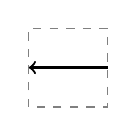
\begin{tikzpicture}
                \draw[dashed,white!50!black] (0,0) rectangle (1,1);
                \draw[thick,->] (1,0.5) -- (0,0.5);
            \end{tikzpicture}
        }
        \wrongchoice{
            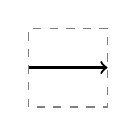
\begin{tikzpicture}
                \draw[dashed,white!50!black] (0,0) rectangle (1,1);
                \draw[thick,->] (0,0.5) -- (1,0.5);
            \end{tikzpicture}
        }
        \wrongchoice{
            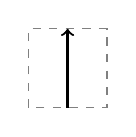
\begin{tikzpicture}
                \draw[dashed,white!50!black] (0,0) rectangle (1,1);
                \draw[thick,->] (0.5,0) -- (0.5,1);
            \end{tikzpicture}
        }
        %% ANS is D
        \correctchoice{
            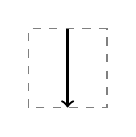
\begin{tikzpicture}
                \draw[dashed,white!50!black] (0,0) rectangle (1,1);
                \draw[thick,->] (0.5,1) -- (0.5,0);
            \end{tikzpicture}
        }
        %% None of the above
    \end{choices}
    \end{multicols}
\end{question}
}

\element{ap}{
\begin{question}{projectile-motion-q31}
    A baseball player throws a ball horizontally.
    Which statement best describes the ball's motion after it is thrown?
    [Neglect the effect of friction.]
    \begin{choices}
        \wrongchoice{Its vertical speed remains the same, and its horizontal speed increases.}
        \wrongchoice{Its vertical speed remains the same, and its horizontal speed remains the same.}
        \wrongchoice{Its vertical speed increases, and its horizontal speed increases.}
      \correctchoice{Its vertical speed increases, and its horizontal speed remains the same.}
        \wrongchoice{Its vertical speed increases and its horizontal speed decreases.}
    \end{choices}
\end{question}
}

\newcommand{\apProjectileMotionQThirtyTwo}{
\begin{tikzpicture}
    %% NOTE: TODO: draw tikz
\end{tikzpicture}
}

\element{ap}{
\begin{question}{projectile-motion-q32}
    %% Base your answers to questions 32 through 34 on
    The following diagram shows a ball of mass $m$ rolled horizontally off a table of height $h$ and landing a distance $D$ from the edge of the table.
    \begin{center}
        \apProjectileMotionQThirtyTwo
    \end{center}
    How much time elapses between the time the ball leaves the edge of the table to when hits the ground?
    \begin{multicols}{3}
    \begin{choices}
        \wrongchoice{$hD$}
        \wrongchoice{$\dfrac{h}{D}$}
        \wrongchoice{$\dfrac{hD}{g}$}
        \wrongchoice{$\dfrac{2h}{g}$}
      \correctchoice{$\sqrt{\dfrac{2h}{g}}$}
    \end{choices}
    \end{multicols}
\end{question}
}

\element{ap}{
\begin{question}{projectile-motion-q33}
    %% Base your answers to questions 32 through 34 on
    The following diagram shows a ball of mass $m$ rolled horizontally off a table of height $h$ and landing a distance $D$ from the edge of the table.
    \begin{center}
        \apProjectileMotionQThirtyTwo
    \end{center}
    What is the initial horizontal velocity of the ball?
    \begin{multicols}{3}
    \begin{choices}
      \correctchoice{$D\sqrt{\dfrac{g}{2h}}$}
        \wrongchoice{$D\sqrt{\dfrac{2h}{g}}$}
        \wrongchoice{$\dfrac{2Dh}{g}$}
        \wrongchoice{$Dhg$}
        \wrongchoice{$\dfrac{g}{Dh}$}
    \end{choices}
    \end{multicols}
\end{question}
}

\element{ap}{
\begin{question}{projectile-motion-q34}
    %% Base your answers to questions 32 through 34 on
    The following diagram shows a ball of mass $m$ rolled horizontally off a table of height $h$ and landing a distance $D$ from the edge of the table.
    \begin{center}
        \apProjectileMotionQThirtyTwo
    \end{center}
    If the initial horizontal velocity of the ball is represented as the quantity $v$,
        what is the kinetic energy of the ball right before it hits the ground?
    \begin{multicols}{2}
    \begin{choices}
        \wrongchoice{$mgh$}
        \wrongchoice{$\dfrac{mv^2}{2}$}
        \wrongchoice{$\dfrac{mv^2 - 2mgh}{2}$}
      \correctchoice{$\dfrac{mv^2 + 2mgh}{2}$}
        \wrongchoice{$\dfrac{2mgh - mv^2}{2}$}
    \end{choices}
    \end{multicols}
\end{question}
}

\element{ap}{
\begin{question}{projectile-motion-q35}
    A person throws a ball at an angle of \ang{30} with the horizontal with a velocity of \SI{32}{\meter\per\second}.
    As the ball is thrown,
        a second person is running past the thrower at a constant velocity.
    At what velocity must this second person run so that she may catch the ball as it hits the ground?
    \begin{multicols}{2}
    \begin{choices}
        \wrongchoice{\SI{32}{\meter\per\second}}
        \wrongchoice{$32\sin\ang{30}\,\si{\meter\per\second}$}
      \correctchoice{$32\cos\ang{30}\,\si{\meter\per\second}$}
        \wrongchoice{$32\tan\ang{30}\,\si{\meter\per\second}$}
        \wrongchoice{$64\cos\ang{30}\,\si{\meter\per\second}$}
    \end{choices}
    \end{multicols}
\end{question}
}

\element{ap}{
\begin{question}{projectile-motion-q36}
    Rocky the Flying Squirrel is carrying a nut of mass \SI{0.5}{\kilo\gram} while flying horizontally at a height of \SI{15}{\meter} above the ground at a speed of \SI{12}{\meter\per\second}.
    Bullwinkle is eagerly awaiting the delivery of the nut on the ground.
    Rocky releases the nut as he is directly above Bullwinkle.
    How far from Bullwinkle will the nut land if Bullwinkle does not move?
    \begin{multicols}{3}
    \begin{choices}
        \wrongchoice{$3\sqrt{2}\,\si{\meter}$}
        \wrongchoice{$3\sqrt{3}\,\si{\meter}$}
        \wrongchoice{$6\sqrt{2}\,\si{\meter}$}
        \wrongchoice{$6\sqrt{3}\,\si{\meter}$}
      \correctchoice{$12\sqrt{3}\,\si{\meter}$}
    \end{choices}
    \end{multicols}
\end{question}
}


\endinput


